\documentclass{article}
\usepackage{ae,aecompl}
\usepackage{todonotes}
\usepackage{chngcntr}
\usepackage{tikz-cd}
\usepackage{graphicx}
\graphicspath{ {./images/}}
\usepackage[all,cmtip]{xy}
\usepackage{amsmath, amscd}
\usepackage{amsthm}
\usepackage{amssymb}
\usepackage{amsfonts}
\usepackage{bm}
\usepackage{qsymbols}
\usepackage{latexsym}
\usepackage{mathrsfs}
\usepackage{mathtools}
\usepackage{cite}
\usepackage{color}
\usepackage{url}
\usepackage{enumerate}
\usepackage{verbatim}
\usepackage[draft=false, colorlinks=true]{hyperref}
\usepackage{pdfpages}
\usepackage[margin=1.2in]{geometry}
\usepackage{IEEEtrantools}
\usepackage{multirow}
\usepackage{fancyhdr}


\usepackage[nameinlink]{cleveref}


\DeclareMathOperator*{\ac}{accept}
\DeclareMathOperator*{\amax}{argmax}
\DeclareMathOperator*{\amin}{argmin}
\DeclareMathOperator*{\Aut}{Aut}
\newcommand {\al}{{\alpha}}
\newcommand {\abs}[1]{{\left\lvert#1\right\rvert}}
\newcommand {\A}{{\mathcal{A}}}
\newcommand {\AM}{{\mathrm{AM}}}
\newcommand {\AMp}{{\AM_{p}^{X}\!(\Ri_\w)}}
\newcommand {\B}{{\mathcal{B}}}
\DeclareMathOperator*{\Be}{Bern}
\newcommand {\Br}{{\dot{B}}}
\newcommand {\Ba}{{\mathfrak{B}}}
\newcommand {\C}{{\mathbb C}}
\newcommand {\ce}{\mathrm{c}}
\newcommand {\Ce}{\mathrm{C}}
\newcommand {\Cc}{\mathrm{C_{c}}}
\newcommand {\Ccinf}{\mathrm{C_{c}^{\infty}}}
\DeclareMathOperator{\DEV}{DEV}
\DeclareMathOperator{\diag}{diag}
\newcommand {\Di}{{\mathbb D}}
\newcommand {\dom}{\mathrm{dom}}
\newcommand {\ud}{\mathrm{d}}
\newcommand {\ue}{\mathrm{e}}
\newcommand {\eps}{\varepsilon}
\newcommand {\veps}{\varepsilon}
\newcommand {\vrho}{{\varrho}}
\newcommand {\E}{{\mathbb{E}}}
\newcommand {\Ec}{{\mathcal{E}}}
\newcommand {\Ell}{L}
\newcommand {\Ellp}{{L_{p}[0,1]}}
\newcommand {\Ellpprime}{{L_{p'}([0,1])}}
\newcommand {\Ellq}{{L_{q}([0,1])}}
\newcommand {\Ellqprime}{{L_{q'}([0,1])}}
\newcommand {\Ellr}{L^{r}}
\newcommand {\Ellone}{{L_{1}([0,1])}}
\newcommand {\Elltwo}{{L_{2}([0,1])}}
\newcommand {\Ellinfty}{L^{\infty}}
\newcommand {\Ellinftyc}{L_{\mathrm{c}}^{\infty}}
\newcommand {\exb}[1]{\exp\left\{#1\right\}}
\DeclareMathOperator*{\Exp}{Exp}
\DeclareMathOperator*{\Ext}{Ext}
\newcommand {\F}{{\mathcal{F}}}
\newcommand{\Fe}{{\mathbb{F}}}
\newcommand
{\G}{{\mathcal{G}}}
\newcommand {\HF}{\mathcal{H}_{\text{FIO}}^{1}(\Rd)}
\newcommand {\Hr}{H}
\newcommand {\HT}{\mathcal{H}}
\newcommand {\ui}{\mathrm{i}}
\newcommand {\I}{{I}}
\newcommand {\J}{{\mathcal{J}}}
\newcommand {\id}{{\mathrm{id}}}
\newcommand {\iid}{\stackrel{\mathclap{\normalfont\mbox{iid}}}{\sim}}
\newcommand {\im}{{\text{im }}}
\newcommand {\ind}{{\perp\!\!\!\perp}}
\newcommand{\indep}{\stackrel{\text{Indep}}{\sim}}
\DeclareMathOperator*{\Int}{int}
\newcommand {\intx}{{\overline{\int_{X}}}}
\newcommand {\inte}{{\overline{\int_{\E}}}}
\newcommand {\la}{\lambda}
\newcommand {\rb}{\rangle}
\newcommand {\lb}{{\langle}}
\newcommand {\La}{\Lambda}
\newcommand {\calL}{{\mathcal{L}}}
\newcommand {\lp}{{\mathcal{L}}^{p}}
\newcommand {\lpo}{{\overline{\mathcal{L}}^{p}\!}}
\newcommand {\Lpo}{{\overline{\Ell}^{p}\!}}
\newcommand {\M}{{\mathbf{M}}}
\newcommand {\Ma}{{\mathcal{M}}}
\newcommand {\N}{{{\mathbb N}}}
\newcommand {\Na}{{{\mathcal{N}}}}
\newcommand {\norm}[1]{\left\|#1\right\|}
\newcommand {\normm}[1]{{\left\vert\kern-0.25ex\left\vert\kern-0.25ex\left\vert #1 
    \right\vert\kern-0.25ex\right\vert\kern-0.25ex\right\vert}}
\newcommand {\Om}{{{\Omega}}}
\newcommand {\one}{{{\bf 1}}}
\newcommand {\pic}{\text{Pic }}
\newcommand {\ph}{{\varphi}}
\newcommand {\Pa}{{\mathbb{P}}}
\newcommand {\Po}{{\mathcal{P}}}
\newcommand {\Q}{{\mathbb{Q}}}
\newcommand {\R}{{\mathbb R}}
\newcommand {\Rd}{{\mathbb{R}^{d}}}
\DeclareMathOperator{\rej}{reject }
\newcommand {\Rn}{{\mathbb{R}^{n}}}
\newcommand {\cR}{{\mathcal{R}}}
\newcommand {\Rad}{{\mathrm{Rad}}}
\newcommand {\ran}{{\mathrm{ran}}}
\newcommand {\Ri}{{\mathrm{R}}}
\newcommand {\supp}{{\mathrm{supp}}}
\newcommand {\Se}{\mathrm{S}}
\newcommand {\Sp}{S^{*}(\Rn)}
\newcommand {\St}{{\mathrm{St}}}
\newcommand {\Sw}{\mathcal{S}}
\newcommand {\T}{{\mathcal{T}}}
\newcommand {\ta}{{\theta}}
\newcommand {\Ta}{{\Theta}}
\DeclareMathOperator {\V}{Var}
\newcommand {\w}{{\omega}}
\newcommand {\W}{{\mathrm{W}}}
\newcommand {\Wnp}{\text{$\mathrm{W}$\textsuperscript{$n,\!p$}}}
\newcommand {\Wnpeq}{\text{$\mathrm{W}$\textsuperscript{$n\!,\!p$}}}
\newcommand {\Wonep}{\text{$\mathrm{W}$\textsuperscript{$1,\!p$}}}
\newcommand {\Wonepeq}{\text{$\mathrm{W}$\textsuperscript{$1\!,\!p$}}}
\newcommand {\X}{{\mathcal{X}}}
\newcommand {\Z}{{{\mathbb Z}}}
\newcommand {\Za}{{\mathcal{Z}}}
\newcommand {\Zd}{{\Z[\sqrt{d}]}}
\newcommand {\vanish}[1]{\relax}

\newcommand {\wh}{\widehat}
\newcommand {\wt}{\widetilde}
\newcommand {\red}{\color{red}}

% Distributions
\newcommand{\normal}{\mathsf{N}}
\newcommand{\poi}{\mathsf{Poisson}}
\newcommand{\bern}{\mathsf{Bernoulli}}
\newcommand{\bin}{\mathsf{Binomal}}
\newcommand{\multi}{\mathsf{Multinomial}}




% put your command and environment definitions here




% some theorem environments
% remove "[theorem]" if you do not want them to use the same number sequence


  \newtheorem{thrm}{Theorem}
  \newtheorem{lemma}{Lemma}
  \newtheorem{prop}{Proposition}
  \newtheorem{cor}{Corollary}

  \newtheorem{conj}{Conjecture}
  \renewcommand{\theconj}{\Alph{conj}}  % numbered A, B, C etc

  \theoremstyle{definition}
  \newtheorem{defn}{Definition}
  \newtheorem{ex}{Example}
  \newtheorem{exs}{Examples}
  \newtheorem{question}{Question}
  \newtheorem{remark}{Remark}
  \newtheorem{notn}{Notation}
  \newtheorem{exer}{Exercise}




\title{STATS300A - Lecture 19}
\author{Dominik Rothenhaeusler\\ Scribed by Michael Howes}
\date{12/01/21}

\pagestyle{fancy}
\fancyhf{}
\rhead{STATS300A - Lecture 19}
\lhead{12/01/21}
\rfoot{Page \thepage}

\begin{document}
\maketitle
\tableofcontents
\section{Announcements}
A practice exam will be posted online today. It is designed to take 3 hours like the final exam.
\section{Set up}
Recall that we have been studying multiple testing. Thus we have data $X \sim \Pa \in \Po$ where $\Pa$ is unknown. For each $i=1,\ldots,n$, we have a null hypothesis $H_{0,i} \subseteq \Po$ and a p-value $p_i(X) \in [0,1]$ such, under $H_{0,i}$
\[\Pa(p_i(X) \le t) \le t, \]
for all $t \in [0,1]$. Our objects of study are decision procedures $\Phi : [0,1]^n \to \{0,1\}^n$ where the input of $\Phi$ is our $n$ p-values $p= (p_1,\ldots,p_n)$ and 
\[\Phi_i(p) = \begin{cases}
    1 & \text{if we reject $H_{0,i}$ based on the p-values $p$},\\
    0 & \text{if we accept $H_{0,i}$ based on the p-values $p$}.
\end{cases} \]
For a given decision procedure $\Phi$ we define two random varaibles $V$ and $R$, where
\begin{align*}
    V &= \# \text{ of false discoveries}\\
    &=\# \text{ of nulls $H_{0,i}$ which are true and are rejected by $\Phi$}\\
    &=\sum_{i:H_{0,i}}\Phi_i,
\end{align*}
where the subscript ${i\!:\!H_{0,i}}$ means that we sum over all indices $i$ such that the null $H_{0,i}$ is true. Likewise we have,
\begin{align*}
    R&=\# \text{ of rejections}\\
    &=\# \text{ of $i$ with $\Phi_i=1$},\\
    &=\sum_{i=1}^n \Phi_i.
\end{align*}
We then defined two quantities which we wanted to control
\[FWER = \Pa(V \ge 1) ~~~\text{and}~~~ FDR = \E\left[\frac{V}{\max\{R,1\}}\right] \]
Last time we looked at the Bonferroni and Holm's procedure which both control $FWER$ but are quite conservative. Today we will see some less conservative methods that allow us to reject more nulls while still gaurding against making too many false rejections. 



\section{Controling $FWER$}
\subsection{Closed testing}
We will first introduce some notation. For $I \subseteq \{1,\ldots,n\}$, define $H_{0,I}=\bigcap_{i \in I}H_{0,i}$. 
\begin{ex}
    Suppose we have $X \sim \Na(\mu,I_3)$ where $\mu \in \R^3$ is unknown and $I_3 \in \R^{3\times 3}$ is the identity matrix. Suppose we have nulls $H_{0,i}:\mu_i=0$ for $i=1,2,3$. Then $H_{0,\{1,2\}}:\mu_1=\mu_2=0$ and $H_{0,\{1,2,3\}} : \mu_1=\mu_2=\mu_3=0$. 
\end{ex}
\begin{defn}
    Suppose that for each $I \subseteq \{1,\ldots,n\}$, we have a level $\al$-test $\phi_I$. The \emph{closed testing procedure} is a procedure that simulateneously tests $H_{0,I}$ for all $I \subseteq \{1,\ldots,n\}$. Under the closed testing procedure we reject $H_{0,I}$ if and only if $\phi_J=1$  for all $J \subseteq \{1,\ldots,n\}$ such that $I \subseteq J$.
\end{defn}
That is, when using the closed testing procedure, we reject $H_{0,I}$ if and only if $\phi_J$ rejects for all $J$ that are supersets of $I$. 
\begin{ex}
    Suppose that we have three hypotheses $H_{0,i}$, $i=1,2,3$. The results of the test $\phi_{I}$ might take this form:
    \begin{center}
    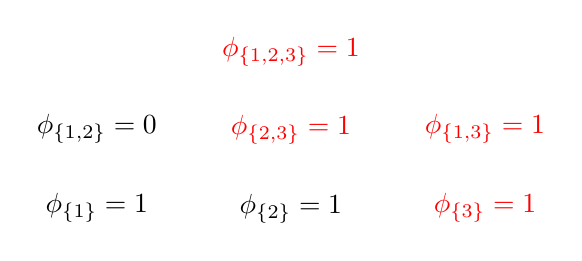
\begin{tikzpicture}
        \node (top) at (0,0) {$\color{red} \phi_{\{1,2,3\}}=1$};
        \node [below left  of=top, xshift = -50, yshift = -8] (left)  {$\phi_{\{1,2\}}=0$};
        \node [below right  of=top, xshift = 50, yshift = -8] (right)  {$\color{red} \phi_{\{1,3\}}=1$};
        \node [below of=top] (middle)  {$\color{red} \phi_{\{2,3\}}=1$};
        \node [below of=left] (leftb)  {$\phi_{\{1\}}=1$}; 
        \node [below of=right] (rightb)  {$\color{red} \phi_{\{3\}}=1$};
        \node [below of=middle] (middleb)  {$\phi_{\{2\}}=1$};
    \end{tikzpicture}
\end{center}
    Since $\phi_{\{1,2\}}=0$, the closed testing procedure does not reject $H_{0,1}$ or $H_{0,2}$. For every $J$ that contains $3$ we have $\phi_J = 1$ and so $H_{0,3}$ is rejected. The tests in red correspond to nulls that are rejected under the closed testing procedure. The other three nulls are not rejected.
\end{ex}
Note that the closed testing procedure is consistent in the sense that if $I \subseteq I'$ and we reject $H_{0,I}$, then we also reject $H_{0,I'}$ which is a subset of $H_{0,I}$. As presented here, closed testing requires an exponential number of tests $\phi_I$. We will see some examples were we can exploit the structure of our tests and perform fewer tests.
\begin{prop}
    If $\phi_I$ is level $\al$ for all $I \subseteq \{1,\ldots,n\}$, then the closed testing procedure controls the $FWER$ of testing $H_{0,I}, I \subseteq \{1,\ldots, n\}$ at $\al$.
\end{prop}
\begin{proof}
    Let $I_0$ be the set of all $i\in \{1,\ldots,n\}$ such that $H_{0,i}$ is true. If the closed testing procedure falsely rejects $H_{0,I}$ for some $I\subseteq \{1,\ldots,n\}$, then we must have $I \subseteq I_0$ and thus $\phi_{I_0}=\al$. Thus
    \[FWER \le \Pa(\phi_{I_0}=1) \le \al.\qedhere\] 
\end{proof}
\begin{remark}
    One might ask why this method is important.
    \begin{itemize}
        \item Firstly, suppose that $\phi_I$ is a Bonferroni test of $H_{0,i},i \in I$. That is $\phi_I=1$ if and only if $p_i \le \frac{\al}{\abs{I}}$ for some $i \in I$. Then if we apply the closed testing procedure to $\phi_I$, we get Holm's testing procedure which is more powerful than Bonferroni.
        \item Pharmaceutical methods are often based on closed testing procedure since they offer a lot of flexibility. 
    \end{itemize}
\end{remark}
\subsection{Nested hypotheses}
\begin{defn}
 We will say that the hypotheses $H_{0,i}$ for $i=1,\ldots,n$ are \emph{nested} if for all $i$, $H_{0,i}\subseteq H_{0,i+1}$.
\end{defn} 
For example, we may have $H_{0,1}:\mu_1=\mu_2=\mu_3=0$, $H_{0,2} :\mu_1=\mu_2=0$, $H_{0,3}:\mu_1=0$. Note that if $H_{0,i}$ are nested and $I \subseteq \{1,\ldots,n\}$, then $H_{0,I}=H_{0,i_0}$ where $i_0=\min(I)$. Thus the closed testing procedure becomes
\[\text{reject $H_{0,i}$} \Longleftrightarrow \phi_1=\phi_2=\ldots=\phi_i = 1. \]
Thus for nested hypotheses, the closed testing procedure controls $FWER$ at level $\al$ and we only need a linear number of tests.
\subsection{Online $FWER$ control}
Suppose we have a sequence of p-values $p_1,p_2,\ldots,$ that we recieve sequentially. This may be the setting for clinical trials or online experiments. At each step $i$ we want to decide whether to reject $H_{0,i}$ based on $p_1,p_2,\ldots,p_i$.
\begin{prop}
    For a fixed level $\al$, let $\Phi_i = \one_{p_i \le \al_i}$ where $\al_i = \frac{\al}{i^2}\cdot \frac{6}{\pi^2}$. Then the procedure $\Phi$ controls $FWER$ at level $\al$.
\end{prop}
\begin{proof}
    Note that $\sum_{i=1}^\infty \frac{1}{i^2}=\frac{\pi^2}{6}$. Thus
    \begin{align*}
        FWER &= \Pa(V \ge 1)\\
        &\le \E[V]\\
        &=\E\left[\sum_{i:H_{0,i}}\Phi_i\right]\\
        &=\E\left[\sum_{i:H_{0,i}}\one_{p_i\le\al_i}\right]\\
        &=\sum_{i:H_{0,i}}\Pa(p_i\le \al_i)\\
        &\le \sum_{i : H_{0,i}}\al_i\\
        &\le \sum_{i=1}^\infty \al_i\\
        &= \frac{6 \al}{\pi^2}\sum_{i=1}^\infty \frac{1}{i^2}\\
        &=\al.\qedhere
    \end{align*}
\end{proof}
Note that we could have taken any choice of $\al_i$ as long as $\sum_{i=1}^\infty \al_i=\al$. If we assume that the p-values are independent we can get a stronger test,
\begin{prop}
    For a fixed level $\al$, let $\Phi_i = \one_{p_i \le \al_i}$ where $\al_i = 1-(1-\al)^{\gamma_i}$ where $\sum_{i=1}^\infty \gamma_i = 1$. If the p-values $p_i$ are independent, then $\Phi$ control $FWER$ at level $\al$. Furthermore, under the global null $\cap_{i=1}^\infty H_{0,i}$, the procedure $\Phi$ has $FWER$ exactly $\al$.
\end{prop}
Note that the previous procedure does not have $FWER$ exactly $\al$ under the global null. Thus this second online procedure is more powerful but it requires an independence assumption.
\begin{proof}
    Note that
    \begin{align*}
        \Pa(V=0) &=\Pa(p_i \ge \al_i, \text{ for all }i:H_{0,i})\\
        &=\prod_{i:H_{0,i}}\Pa(p_i\ge \al_i)\\
        &= \prod_{i:H_{0,i}}(1-\al_i)\\
        &=\prod_{i:H_{0,i}}(1-\al)^{\gamma_i}\\
        &=(1-\al)^{\sum_{i:H_{0,i}}\gamma_i}\\
        &\ge (1-\al)^{\sum_{i=1}^\infty \gamma_i}\\
        &=1-\al,
    \end{align*}
    and we have equality under the global null. Thus 
    \[FWER =  1-\Pa(V=0) \le 1-(1-\al)=\al,\]
    and again we have equality under the global null.
\end{proof}
\section{$FDR$ control}
We will now briefly talk about $FDR$ control. This will be discussed in more detail in 300C with Professor Candes. Recall that 
\[FDR = \E\left[\frac{V}{\max\{R,1\}}\right]. \]
We observed last lecture that
\[FDR \le FWER,\]
thus controlling $FDR$ instead of $FWER$ allows for more powerful procedures.
\begin{remark}
    Some people prefer to work directly with $FDP = \frac{V}{\max\{R,1\}}$. Instead of controlling $FDR=\E[FDP]$, these people wish to control $\Pa(FDP \ge c)$.
\end{remark} 
\begin{defn}[Benjamini-Hochberg procedure]
    Fix $q \in [0,1]$. First order our p-values $p_{(1)}\le p_{(2)} \le \ldots \le p_{(n)}$ and sort the corresponding nulls $H_{0,(1)},H_{0,(2)},\ldots,H_{0,(n)}$. Let $i_0$ be the largest $i$ such that 
    \[p_{(i)} \le \frac{i}{n}q. \]
    The \emph{Benjamini-Hochberg procedure} (BH) rejects all nulls $H_{0,(i)}$ for $i=1,\ldots,i_0$.
\end{defn}
In partice $q=0.1$ is a popular threshold.
\begin{prop}
    If the p-values are independent, then the Benjamini-Hochberg procedure controls $FDR$ at level $q$.
\end{prop}
\begin{proof}
    Let $\Phi$ be the decision procedure from $BH$. For each $i,k=1,\ldots,n$, define an event $C_k^{(i)}$ as follows 
    \[C_k^{(i)} = \left\{\sum_{j=1}^n \Phi_j(p_1(X),\ldots,p_{i-1}(X),0,p_{i+1}(X),\ldots,p_n(X))=k  \right\}. \]
    Thus $C_k^{(i)}$ is the event when $BH$ would reject exactly $k$ hypotheses if we fixed $p_i=0$. Note that since our p-values are independent, $p_i$ is independent of $C_k^{(i)}$ for all $i$ and $k$. 

    Without loss of generality, we can reorder $H_{0,i}$ so that 
    \[H_{0,1},\ldots,H_{0,n_0} \text{ are true}, \]
    and
    \[H_{0,n_0+1},\ldots, H_{0,n} \text{ are false.} \]
    Thus $V = \sum_{i=1}^{n_0}\Phi_i$ and if $R \neq 0$, then $\frac{1}{R}=\sum_{k=1}^n \frac{1}{k}\one_{R=k}$. Thus
    \begin{align*}
        FDR &= \sum_{k=1}^n \frac{1}{k}\E[\one_{R=k}V]\\
        &=\sum_{k=1}^n \sum_{i=1}^{n_0}\frac{1}{k}\E[\one_{R=k}\Phi_i]\\
        &=\sum_{k=1}^n \sum_{i=1}^{n_0}\frac{1}{k} \Pa(R=k \text{ and } \Phi_i = 1)\\
        &=\sum_{k=1}^n \sum_{i=1}^{n_0}\frac{1}{k} \Pa\left(R=k \text{ and } p_i \le \frac{k}{n}q\right).
    \end{align*}
    Note that 
    \[\left\{R=k \text{ and } p_i \le \frac{k}{n}q\right\} = C_k^{(i)}\cap\left\{p_i \le \frac{k}{n}q\right\}. \]
    This is because requiring that $R=k$ and $p_i \le \frac{k}{n}q$ is equivalent to $p_i \le \frac{k}{n}q$ and requiring that $R=k$ if $p_i=0$. Thus we have
    \begin{align*}
        FDR &= \sum_{k=1}^n \sum_{i=1}^{n_0}\frac{1}{k} \Pa\left(C_k^{(i)}\cap\left\{p_i \le \frac{k}{n}q\right\}\right)\\
        &=\sum_{k=1}^n \sum_{i=1}^{n_0} \frac{1}{k} \Pa\left(C_k^{(i)}\right)\Pa\left(p_i \le \frac{k}{n}q\right)\\
        &=\sum_{k=1}^n \sum_{i=1}^{n_0} \frac{q}{n} \Pa\left(C_k^{(i)}\right)\\
        &=\frac{q}{n}\sum_{i=1}^{n_0}\sum_{k=1}^n\Pa\left(C_k^{(i)}\right).
    \end{align*}
    For each $i$, if $p_i =0$, then $R\ge 1$. Thus, for each $i$, our sample space is the disjoint union of $C_k^{(i)}$ for $k=1,\ldots,n$. Thus
    \begin{align*}
        FDR &= \frac{q}{n}\sum_{i=1}^{n_0}\sum_{k=1}^n\Pa\left(C_k^{(i)}\right)\\
        &=\frac{q}{n}\sum_{i=1}^{n_0}1\\
        &=\frac{qn_0}{n}\\
        &\le q \qedhere
    \end{align*}
\end{proof}
\end{document}